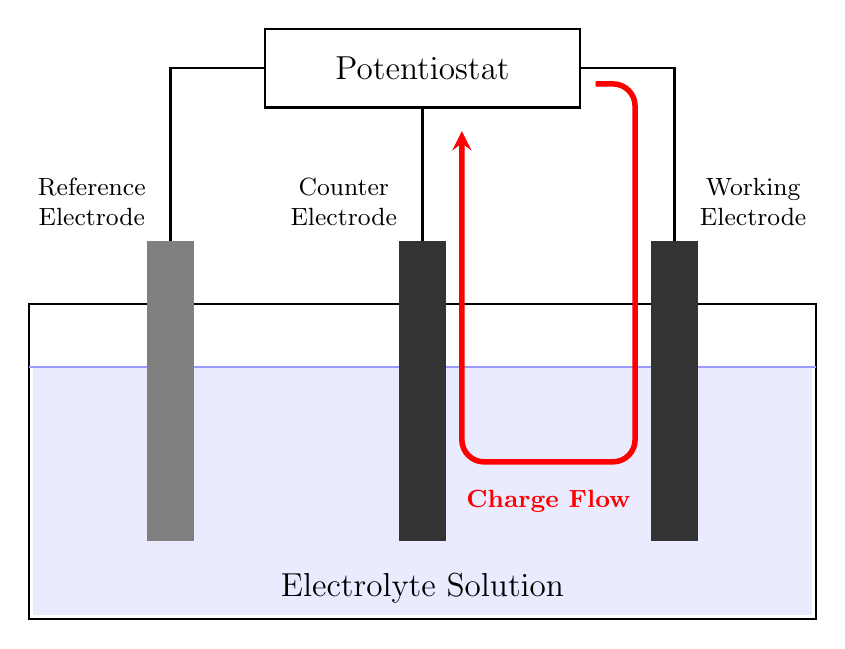
\begin{tikzpicture}[>=stealth, thick]

  % Solution vessel
  \draw[thick] (0, 0) -- (0, 4) -- (10, 4) -- (10, 0) -- cycle;
  % Solution fill
  \fill[blue!8] (0.05, 0.05) rectangle (9.95, 3.2);
  % Solution surface line
  \draw[blue!40, thick] (0, 3.2) -- (10, 3.2);
  \node[font=\large] at (5, 0.4) {Electrolyte Solution};

  % Potentiostat box
  \draw[thick, fill=white] (3, 6.5) rectangle (7, 7.5);
  \node[font=\large] at (5, 7) {Potentiostat};

  % Reference Electrode (left)
  \fill[black!50] (1.5, 1.0) rectangle (2.1, 4.8);
  \node[font=\small, align=center] at (0.8, 5.3) {Reference\\Electrode};
  % Wire from counter electrode to potentiostat
  \draw[thick] (1.8, 4.8) -- (1.8, 7) -- (3, 7);

  % Counter Electrode (centre)
  \fill[black!80] (4.7, 1.0) rectangle (5.3, 4.8);
  \node[font=\small, align=center] at (4.0, 5.3) {Counter\\Electrode};
  % Wire from reference electrode to potentiostat
  \draw[thick] (5.0, 4.8) -- (5.0, 6.5);

  % Working Electrode (right)
  \fill[black!80] (7.9, 1.0) rectangle (8.5, 4.8);
  \node[font=\small, align=center] at (9.2, 5.3) {Working\\Electrode};
  % Wire from working electrode to potentiostat
  \draw[thick] (8.2, 4.8) -- (8.2, 7) -- (7, 7);

  % Charge flow arrows (red loop)
  \draw[->, red, line width=2pt, rounded corners=8pt]
  (7.2, 6.8) -- (7.7, 6.8) -- (7.7, 2.0) -- (5.5, 2.0)
  -- (5.5, 4.0) -- (5.5, 6.2);
  \node[red, font=\small\bfseries] at (6.6, 1.5) {Charge Flow};

\end{tikzpicture}
